\section{Equal-Budget Benchmark Protocol and Surrogate Framework}
\label{sec:protocol}

\subsection{Surrogate Ensemble and Cross-Validation}
The active-learning loop uses an ensemble of $M = 5$ multi-layer perceptrons (scikit-learn \texttt{MLPRegressor}), each with two hidden layers of 64 rectified-linear units, trained with Adam for at most 1{,}000 epochs with early stopping on a held-out $10\%$ of the training data. Inputs are scaled to $[0, 1]$ and outputs are standardized. Each network predicts five quantities jointly: $C_L$, $C_D$, $L/D$, the calm-air range $R$ and the soft-penalty score of Section~\ref{sec:formulation}. The ensemble is fitted on feasible designs only, because infeasible designs carry no aerodynamic outputs. The five members differ only in their random seed ($42, 101, 2024, 777, 999$ in the original campaign; $42 + 7s + 100i$, $i = 0,\ldots,4$, in replication $s$). The prediction and its uncertainty are the ensemble mean and standard deviation,
\begin{equation}
\bar{\mu}_y(\mathbf{x}) = \frac{1}{M} \sum_{m=1}^M \hat{y}_m(\mathbf{x}), \qquad \bar{\sigma}_y(\mathbf{x}) = \sqrt{\frac{1}{M} \sum_{m=1}^M \big(\hat{y}_m(\mathbf{x}) - \bar{\mu}_y(\mathbf{x})\big)^2} .
\end{equation}
Five-fold cross-validation on the feasible designs of the database gives $R^2 \ge 0.996$ for every target and a mean absolute percentage error of $2.3\%$ for range (Table~\ref{tab:cv}). These are in-distribution figures; Section~\ref{sec:distribution_shift} shows that accuracy is much lower on the designs that the loop itself proposes.

\subsection{Feasibility Classifier and Recall Audit}
\label{sec:classifier_audit}
About $72\%$ of the space-filling pool is infeasible. A random forest classifier with $100$ trees~\cite{breiman2001random} is therefore trained on all evaluated designs, feasible or not, to predict a probability of feasibility $\mathcal{P}_{\mathrm{feas}}(\mathbf{x}) \in [0, 1]$, which weights the acquisition function below. An infeasible design returns no aerodynamic outputs, so from the point of view of the search the constraints act as what the simulation-optimization literature calls hidden constraints~\cite{ledigabel2015taxonomy}, and a model of the probability that an evaluation succeeds is the usual way to handle them in surrogate-based aircraft design~\cite{bussemaker2024hidden}.

The held-out performance of this classifier was audited on the $\NclfNrows$-evaluation database with five repeated stratified 80/20 random splits (seeds 0 to 4) and one scaled-feature forest (Table~\ref{tab:classifier_audit}):
\begin{itemize}
    \item \textbf{Global and frontier recall.} Precision is $\NfnPrec\% \pm \NfnPrecSd\%$ and recall is $\NfnRecall\% \pm \NfnRecallSd\%$ at a threshold of $0.5$ (the same forest without feature scaling gives $\NfnRecallUnscaled\%$ recall); $\NclfInfeasShare\%$ of the audited designs are infeasible. Recall is higher among good designs: $\NfnTenRecall\% \pm \NfnTenRecallSd\%$ among the top 10\% of valid designs ($R \ge \NclfQten\,\mathrm{km}$) and $\NfnTwoRecall\% \pm \NfnTwoRecallSd\%$ among the top 2\% ($R \ge \NclfQtwo\,\mathrm{km}$), the latter on only \NfnTwoN\ designs per split.
    \item \textbf{Where the false negatives lie.} $\NfnWithin\%$ of the falsely rejected valid designs lie within $10\%$ of the static-margin or trim limits, against $\NtpWithin\%$ of the correctly accepted ones. Their median range is $\NfnMedian\,\mathrm{km}$ (accepted: $\NtpMedian\,\mathrm{km}$), but the best falsely rejected design averages $\NfnMax\,\mathrm{km}$ over the splits (maximum $\NfnMaxSplit\,\mathrm{km}$). The decision boundary therefore passes close to the best designs, and a hard gate at $0.5$ would exclude some of them.
    \item \textbf{What the classifier cannot see.} The forest is trained on axis-aligned splits of the raw design variables. The washout rule $g_8$ is a relation between four variables, and Section~\ref{sec:budget_results} shows that the classifier-weighted search still proposes designs that violate it.
\end{itemize}

\subsection{Acquisition Function and Active-Learning Loop}
\label{sec:al_loop}
Candidates are ranked by an upper confidence bound on range~\cite{srinivas2012information}, weighted by the classifier~\cite{gelbart2014bayesian} and reduced by the predicted soft penalty:
\begin{equation}
a(\mathbf{x}) = \big( \bar{\mu}_R(\mathbf{x}) + \kappa\, \bar{\sigma}_R(\mathbf{x}) \big)\, w\!\big(\mathcal{P}_{\mathrm{feas}}(\mathbf{x})\big) - \max\!\big(0, \bar{\mu}_{\pi}(\mathbf{x})\big), \qquad w(p) = \frac{1}{1 + e^{-10\,(p - 0.5)}} ,
\label{eq:ucb_acquisition}
\end{equation}
with $\kappa = 0.3$ in the original campaign and in every run reported here. The weight $w$ is a sigmoid of the classifier probability; it equals $0.5$ at $\mathcal{P}_{\mathrm{feas}} = 0.5$ and saturates toward $0$ and $1$. Probability-of-feasibility weighting of this kind has known limitations~\cite{cordelier2026multifidelity}, and Section~\ref{sec:feas_ablation} tests it by replacing $w$ with a hard $0/1$ gate at $0.5$ and by removing it ($w \equiv 1$).

One cycle of the loop proceeds as follows. (i) The ensemble is refitted on all feasible designs and the classifier on all designs evaluated so far, including the pool. (ii) The acquisition $a(\mathbf{x})$ is maximized over the box of Table~\ref{tab:design_bounds} by differential evolution (SciPy, population $150 \times 14 = 2{,}100$, at most 300 generations, initial population seeded with the 20 best feasible designs, followed by the default local polish). (iii) From the final population, the five distinct members with the highest acquisition and one further member with the largest weighted uncertainty $\bar{\sigma}_R\, w$ are taken as candidates; candidates that duplicate an evaluated design are dropped. (iv) The candidates are evaluated with the full pipeline and added to the data. The loop therefore proposes up to six designs per cycle and retrains every cycle. The original campaign ran this loop until a wall-clock limit, which it reached after 287 evaluations; the replications run it for exactly 287 evaluations instead, so that every strategy has the same budget.

\subsection{Equal-Budget Protocol}
\label{sec:budget_protocol}
Figure~\ref{fig:protocol} summarizes the benchmark. Every strategy starts from the same pool of 9{,}800 Latin hypercube designs (best range $352.9\,\mathrm{km}$, $28.1\%$ feasible) and may spend $287$ further evaluations of the full pipeline. A run is one strategy with one random seed. The strategies are:
\begin{enumerate}
    \item \textbf{Active learning as published (AL).} The loop of Section~\ref{sec:al_loop}, ten replications (seeds 0 to 9) plus the original campaign. The published loop evaluates the candidates exactly as the differential evolution returns them.
    \item \textbf{Active learning with washout repair (AL-R).} The same loop, except that the four twist variables of each candidate are sorted into the order required by $g_8$ before the duplicate check and the evaluation (\NvNALR\ seeds). Every other strategy below, and the pool itself, already applies this sorting; Section~\ref{sec:budget_results} explains why this arm was added.
    \item \textbf{Trust-region Bayesian optimization (TuRBO).} A TuRBO-1 implementation~\cite{eriksson2019turbo}: a Gaussian process (Mat\'ern-$5/2$ kernel with automatic relevance determination) is fitted to at most 400 designs inside a trust region centered on the best feasible design, with infeasible designs assigned the worst feasible value in the region; batches of six are chosen by Thompson sampling over 2{,}000 Sobol candidates with the TuRBO perturbation mask; the region side (initially $0.4$ of the normalized range) doubles after three consecutive improving batches, halves after five consecutive failures and restarts below $0.01$ (\NvNTurbo\ seeds).
    \item \textbf{Adaptive local search (adapt10).} No surrogate. Each batch of six consists of Gaussian perturbations, with a standard deviation of $10\%$ of each variable's range, of randomly chosen members of the current 20 best feasible designs (pool and new evaluations together), so that the set of parents moves as better designs are found (\NvNAdapt\ seeds). This arm has the same batch structure and the same parent set as the active-learning loop but replaces the surrogate-optimized proposals by random ones.
    \item \textbf{Static local search (local10, local5).} Gaussian perturbations ($10\%$ or $5\%$ of the range) of randomly chosen members of the 20 best pool designs; the parent set never changes (10 seeds each).
    \item \textbf{Fresh Latin hypercube and uniform random sampling.} 287 new space-filling or uniform samples in the full box (10 seeds each).
\end{enumerate}
Section~\ref{sec:pool_size} repeats TuRBO, adapt10 and AL-R from random subsamples of 288, 1{,}000 and 3{,}000 pool designs. Three further arms isolate the classifier weight (Section~\ref{sec:feas_ablation}): active learning with a hard gate, active learning without the weight (each with and without the washout repair where stated), and TuRBO with the sigmoid weight applied to its Thompson samples.

\begin{figure}[htbp]
\centering
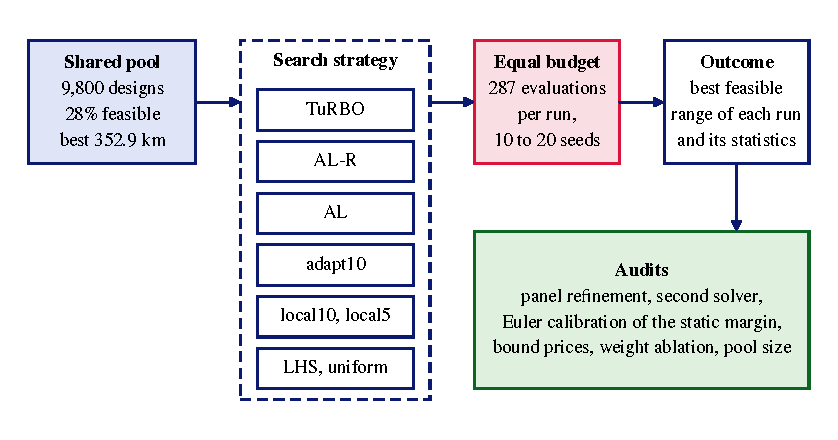
\includegraphics[width=\linewidth]{figures/fig_protocol.pdf}
\caption{Structure of the benchmark. All strategies share the pool, the evaluator and the budget; they differ only in how the 287 further designs are proposed. The audits are reported in Section~\ref{sec:results}.}
\label{fig:protocol}
\end{figure}

\paragraph{Two corrections made during the audit of the benchmark code} Both are reported because they change numbers, and the runs made before each correction are retained and listed in Table~\ref{tab:asrun}. First, the published active-learning loop was the only strategy that did not sort the twist variables, so it alone spent evaluations on designs that fail $g_8$; the AL-R arm removes that asymmetry. Second, the first implementations of TuRBO and of the adaptive local search compared the ranges of new evaluations and of pool designs on two different energy bases (a constant factor of $1.30$ in favor of new designs), which distorted the choice of the trust-region center and of the parent set. Both strategies were rerun with one consistent basis, and the corrected runs are the ones reported as TuRBO and adapt10. The weighting and bound-price experiments of Sections~\ref{sec:feas_ablation} and~\ref{sec:bound_prices}, first made with the first TuRBO implementation, were repeated with the corrected one, and the repeated runs are the ones reported.

\paragraph{Statistics} The outcome of a run is its best feasible range after 287 evaluations. An active-learning run ends early if 40 consecutive cycles produce no candidate that has not already been evaluated; such a run keeps the best value it reached and is not excluded (one AL run stopped at 117 evaluations and one AL-R run at 83). Strategies are compared with two-sided Welch $t$-tests and two-sided Mann--Whitney $U$ tests on these values, and with a percentile bootstrap interval ($20{,}000$ resamples) on the difference of means. For the \NvNfamily\ headline comparisons of Table~\ref{tab:tests} the Welch $p$-values are also reported after Holm correction. A non-significant difference is not read as equivalence; the confidence interval states which differences remain possible. All ranges are on the $\NeU\,\mathrm{Wh/kg}$ basis.
